\documentclass[conf]{new-aiaa}
%\documentclass[journal]{new-aiaa} for journal papers
\usepackage[utf8]{inputenc}

\usepackage{graphicx}
\usepackage{amsmath}
\usepackage[version=4]{mhchem}
\usepackage{siunitx}
\usepackage{longtable,tabularx}
\setlength\LTleft{0pt} 

\usepackage{lipsum}  
\usepackage{svg}
\usepackage{booktabs}

\title{Utilizing Statistical Learning Algorithm to Solve Problems in Aerospace Engineering}

\author{Hafizh Renanto Akhmad\footnote{13621060, Undergraduate Student, Faculty of Mechanical and Aerospace Engineering}, Abisatya Hadyan Dhananjaya\footnote{Undergraduate Student, Faculty of Mechanical and Aerospace Engineering}, Isna Nur Firdausi\footnote{Undergraduate Student, Faculty of Mechanical and Aerospace Engineering}, and Rizky Amalis Zhuraida\footnote{Undergraduate Student, Faculty of Mechanical and Aerospace Engineering}}
\affil{Institut Teknologi Bandung, Bandung, Jawa Barat, 40132}

\begin{document}

\maketitle

\begin{abstract}
\lipsum[1]
\end{abstract}

\section{Nomenclature}

{\renewcommand\arraystretch{1.0}
\noindent\begin{longtable*}{@{}l @{\quad=\quad} l@{}}
    $M$ & Mach number\\
    $V_f$ & Flutter speed\\
    $DC$ & Damping coefficient
\end{longtable*}}

\section{Introduction}
\lettrine{T}{he} 

\section{Statistical Learning}
\subsection{Definition}
Statistical learning referes to the set approaches or methods to estimate a function relating a set of inputs and a set of outputs based on a set of known datas. Suppose we have a set of inputs (or features) $X$ and a set of outputs (or responses) $Y$. There exists a fixed, unknown function $f$ representing the relationship between $X$ and $Y$ such that 
\begin{equation} \label{eq:statslearndef}
    Y = f(X) + \epsilon
\end{equation}
where $\epsilon$ is a random error term, which is independent of $X$ and has mean zero. $f$ represents the systematic information that $X$ provides about $Y$ [1]. Statistical learning is a set of approaches to estimate $f$ based on some given data.

\subsection{Main Purpose}
There are two main purposes in using statistical learning to estimate $f$: prediction and inference. Suppose we already have a set of inputs $X_k$ and its corresponding outputs $Y_k$. At some point, we may have a set of inputs $X_u$ but we do not have the corresponding outputs $Y_u$. This is where the need of prediction rises. We may use statistical learning to estimate $f$ using $X_k$ and $Y_k$ and using the results to predict $Y_u$. As $\epsilon$ averages to zero, we may have
\begin{equation} \label{eq:statslearnpred}
    \hat{Y} = \hat{f}(X)
\end{equation}
where $\hat{f}$ represents the estimate of $f$ and $\hat{Y}$ represents the prediction of $Y$. Here, we may say $\hat{f}$ is our model. On the other hand, we may wish to understand how $Y$ is affected by $X$ as $X$ changes. Here, we wish to estimate $f$ but not for the purpose of prediction. Using Statistical learning, we may infer the relationship between $X$ and $Y$ by estimating $f$ using $X_k$ and $Y_k$. Therefore, our main goal is to apply statistical learning to $X_k$ and $Y_k$, known as the training data, in order to estimate $f$, resulting in our model of $\hat{f}$. We may then use the resulting model to predict $Y_u$ or to infer the relationship between $X$ and $Y$.

\subsection{Regression vs Classification}
There are two types of problems in statistical learning: regression and classification. In regression problems, the response $Y$ is quantitative, while in classification problems, the response $Y$ is qualitative or categorical. In this report, we will utilize three basic statistical learning methods: linear regression for regression problems, logistic regression for classification problems, and K-Nearest Neighbors algorithm for both regression and classification problems, to solve some problem cases in aerospace engineering.

\subsection{Linear Regression}
\subsubsection{Definition}
Linear regression is a very simple approach in statistical learning. It is classified as a parametric method, which means that it makes an assumption about the functional form, or shape, of $f$, and a supervised learning, which means that it uses a set of labeled datas, and is used for regression problems. Linear regression assumes that there exists a linear relationship between $X = (X_1, X_2, \dots, X_p)$ and $Y$, which means that $f$ can be expressed as
\begin{equation} \label{eq:linmod}
    f(X) = \beta_0 + \beta_1X_1 + \beta_2X_2 + ... + \beta_pX_p
\end{equation}
where $X_j$ represents the $j$th feature of $X$ and $\beta_j$ represents the $j$th coefficient of $f$. $\beta_j$ quantifies the relation between $X_j$ and $Y$, which can be interpreted as average effect on $Y$ of a one unit increase in $X_j$, holding other predictors fixed. The values of $\beta_j$ are unknown and must be estimated based on the training data. Suppose $\hat{\beta}_0, \hat{\beta}_1, \dots, \hat{\beta}_p$ are the estimates of $\beta_0, \beta_1, \dots, \beta_p$, respectively, we may have our estimate of $Y$ as
\begin{equation} \label{eq:linreg}
    \hat{Y} = \hat{\beta}_0 + \hat{\beta}_1X_1 + \hat{\beta}_2X_2 + ... + \hat{\beta}_pX_p
\end{equation}

When $p = 1$, the linear regression model is called a simple linear regression model, otherwise, it is called a multiple linear regression model.

\subsubsection{Estimating the Coefficients}
The most common approach to estimate the coefficients is Ordinary Least Squares (OLS). OLS chooses $\hat{\beta}_0, \hat{\beta}_1, \dots, \hat{\beta}_p$ to minimize the residual sum of squares (RSS), which is defined as 
\begin{equation} \label{eq:rss}
    \textrm{RSS}\left(\hat{\beta}_0, \hat{\beta}_1, \dots, \hat{\beta}_p\right) = \sum_{i=1}^{n} \left(y_i - \hat{y}_i\right)^2 = \sum_{i=1}^{n} \left(y_i - \hat{\beta}_0 - \hat{\beta}_1x_{i1} - \hat{\beta}_2x_{i2} - ... - \hat{\beta}_px_{ip}\right)^2
\end{equation}
where $n$ is the number of training data. Let
\begin{equation*}
    \mathbf{F} = 
    \begin{bmatrix}
        1 & x_{11} & x_{12} & \dots & x_{1p} \\
        1 & x_{21} & x_{22} & \dots & x_{2p} \\
        \vdots & \vdots & \vdots & \ddots & \vdots \\
        1 & x_{n1} & x_{n2} & \dots & x_{np}
    \end{bmatrix}, \quad
    \mathbf{y} = 
    \begin{bmatrix}
        y_1 \\ y_2 \\ \vdots \\ y_n
    \end{bmatrix}, \quad
    \hat{\boldsymbol{\beta}} =
    \begin{bmatrix}
        \hat{\beta_0} \\ \hat{\beta_1} \\ \vdots \\ \hat{\beta_p}
    \end{bmatrix}
\end{equation*}
and thus \eqref{eq:rss} can be rewritten as
\begin{equation} \label{eq:rssmat}
    \textrm{RSS}\left(\hat{\boldsymbol{\beta}}\right) = \left(\mathbf{y} - \mathbf{F}\hat{\boldsymbol{\beta}}\right)^T\left(\mathbf{y} - \mathbf{F}\hat{\boldsymbol{\beta}}\right)
\end{equation}
The OLS estimates of $\beta_0, \beta_1, \dots, \beta_p$ are the values that minimize RSS, or the values that satisfy
\begin{equation} \label{eq:ols}
    \frac{\partial \textrm{RSS}}{\partial \hat{\boldsymbol{\beta}}} = -2\mathbf{F}^T\left(\mathbf{y} - \mathbf{F}\hat{\boldsymbol{\beta}}\right) = 0
\end{equation}
which gives
\begin{equation} \label{eq:betaval}
    \hat{\boldsymbol{\beta}} = \left(\mathbf{F}^T\mathbf{F}\right)^{-1}\mathbf{F}^T\mathbf{y}
\end{equation}

\subsubsection{Evaluating the Accuracy of the Coefficient Estimates}
For each $\beta_j$, we have to assess its accuracy using a hypothesis test. Before that, we need to calculate each $\textrm{Var}\left(\hat{\beta}_j\right)$, the variance of $\hat{\beta}_j$. As each $\beta_j$ in $\boldsymbol{\beta}$ is a random variable, using the definition of variance and \eqref{eq:betaval}, we have the variance of $\hat{\boldsymbol{\beta}}$ as
\begin{equation} \label{eq:betavar}
    \textrm{Var}\left(\hat{\boldsymbol{\beta}}\right) = \sigma^2 \left(\mathbf{F}^T\mathbf{F}\right)^{-1}
\end{equation}
where $\sigma^2$ is the variance of the error terms $\epsilon$, which can be estimated using
\begin{equation} \label{eq:sigmasq}
    \hat{\sigma}^2 = \frac{1}{n_{\textrm{train}}-p-1} \textrm{RSS}\left(\hat{\boldsymbol{\beta}}\right)
\end{equation}
where $n_{\textrm{train}}$ is the number of training data and $p$ is the number of features. The variance of $\hat{\beta}_j$ is the $j$th diagonal element of \eqref{eq:betavar}. 
After calculating variance for each $\hat{\beta}_j$, they can be tested using the following procedure:
\begin{enumerate}
    \item Calculate the standard error of $\hat{\beta}_j$ using
    \begin{equation} \label{eq:sebetaj}
        \textrm{SE}\left(\hat{\beta}_j\right) = \sqrt{\textrm{Var}\left(\hat{\beta}_j\right)}
    \end{equation}
    \item Determine the significant level $\alpha$ (usually 0.05)
    \item Determine $H_0$ and $H_1$. As we're assessing relation between $\beta_j$ and $y$, $H_0$ is $\beta_j = 0$ and $H_1$ is $\beta_j \neq 0$.
    \item Calculate the $t$-statistic
    \begin{equation} \label{eq:tstat}
        t_j = \frac{\hat{\beta}_j - 0}{\textrm{SE}\left(\hat{\beta}_j\right)}
    \end{equation}
    \item Calculate the $p$-value using the $t$-statistic and the $t$-distribution with $n_\textrm{train}-p-1$ degrees of freedom
    \item Reject $H_0$ if $p$-value $< \alpha$, otherwise fail to reject $H_0$
\end{enumerate}

\subsubsection{Evaluating the Model Fit}
After evaluating each $\beta_j$, we may evaluate the overall model performance. To evaluate how fit is the model with the training data, we may use the $R^2$ score and the RSE score. For linear regression, the $R^2$ score is defined as
\begin{equation} \label{eq:rsq}
    R^2 = \frac{\textrm{TSS} - \textrm{RSS}}{\textrm{TSS}}
\end{equation}
where TSS is the total sum of squares. TSS is defined as
\begin{equation} \label{eq:tss}
    \textrm{TSS} = \sum_{i=1}^{n_{\textrm{train}}} \left(y_i - \bar{y}\right)^2
\end{equation}
where $\bar{y}$ is the mean of $y$. The RSE score is defined as
\begin{equation} \label{eq:rse}
    \textrm{RSE} = \sqrt{\frac{1}{n_{\textrm{train}}-p-1}\textrm{RSS}}
\end{equation}
A good model fit should have a high $R^2$ score and a low RSE score.

\subsection{Logistic Regression}
\subsubsection{Definition}
Logistic or logit regression is another simplest method in staistical learning. It is a classification model that predicts the probability of a data point belonging to a class using the logistic function. The logistic function is defined as
\begin{equation} \label{eq:logistic}
    f(x) = \frac{e^x}{1 + e^x} = \frac{1}{1 + e^{-x}}
\end{equation}
Using \eqref{eq:logistic}, we have the logistic regression model as
\begin{equation} \label{eq:logreg}
    p\left(X\right) = \frac{1}{1 + e^{-\left(\beta_0 + \beta_1 X_1 + \cdots + \beta_p X_p\right)}}
\end{equation}
where $p\left(X\right)$ is the probability of the response of $X$ belonging to a certain class. By manipulating the left-hand side, we may have
\begin{equation} \label{eq:logregmanip}
    \frac{p\left(X\right)}{1 - p\left(X\right)} = e^{\beta_0 + \beta_1 X_1 + \cdots + \beta_p X_p}
\end{equation}
which is called the odds of the data points having a response of the corresponding class. Taking the natural logarithm of both sides, we have
\begin{equation} \label{eq:logreglog}
    \ln\left(\frac{p\left(X\right)}{1 - p\left(X\right)}\right) = \beta_0 + \beta_1 X_1 + \cdots + \beta_p X_p
\end{equation}
which is called the log-odss or logit.

When $p = 1$, the logistic regression model is called the simple logistic regression model. Otherwise, it is called the multiple logistic regression model.

\subsubsection{Estimating the Regression Coefficients}
The regression coefficients $\beta_j$ can be estimated using the maximum likelihood method (MLE). Let 
\begin{equation}
    \boldsymbol{\beta} =
    \begin{bmatrix}
        \beta_0 \\ \beta_1 \\ \beta_2 \\ \vdots \\ \beta_p
    \end{bmatrix}, \quad
    \mathbf{F} = 
    \begin{bmatrix}
        1 & x_1 & x_2 & \dots & x_p
    \end{bmatrix}
\end{equation}
and thus, we may rewrite \eqref{eq:logreg} as
\begin{equation} \label{eq:logregmat}
    p\left(\mathbf{F}\right) = \frac{1}{1 + e^{-\mathbf{F}\boldsymbol{\beta}}}
\end{equation}
The likelihood function is defined as
\begin{equation} \label{eq:logreglike}
    \textrm{L}\left(\boldsymbol{\beta}\right) = \prod_{i:y_i=1} p\left(\mathbf{F}_i\right) \prod_{i':y_{i'}=0} \left(1 - p\left(\mathbf{F}_{i'}\right)\right) = \prod_{i=1}^{n_{\textrm{train}}} p\left(\mathbf{F}_i\right)^{y_i} \left(1 - p\left(\mathbf{F}_i\right)\right)^{1-y_i}
\end{equation}
The MLE method estimates $\beta_0, \beta_1, \cdots, \beta_p$ by maximizing \eqref{eq:logreglike}. However, it is easier to maximize the log-likelihood function. The log likelihood function is defined as
\begin{equation} \label{eq:logregloglike}
    \ln \textrm{L} \left(\boldsymbol{\beta}\right) = \sum_{i=1}^{n_{\textrm{train}}} \left(y_i \mathbf{F_i}\boldsymbol{\beta} - \ln \left(1 + e^{\mathbf{F}_i\boldsymbol{\beta}}\right) \right)
\end{equation}
and its derivative as
\begin{equation} \label{eq:logregloglikeder}
    \frac{\partial \ln \textrm{L} \left(\boldsymbol{\beta}\right)}{\partial \boldsymbol{\beta}} = \sum_{i=1}^{n_{\textrm{train}}} \left(y_i - p\left(\mathbf{F}_i\right)\right) \mathbf{F}_i
\end{equation}
\eqref{eq:logregloglike} is maximized when \eqref{eq:logregloglikeder} is equal to zero. However, there is no closed-form solution for $\boldsymbol{\beta}$, and thus, numerical methods are used to find the solution. 

One of the most popular numerical solution for this problem is the Newton-Raphson method. The Newton-Raphson method is an iterative method that uses the first derivative of a function to find the root of the function. The general form of the Newton-Raphson method is:
\begin{equation} \label{eq:newraph}
    x_{i+1} = x_i - \frac{f(x_i)}{f'(x_i)}
\end{equation}
where $x_i$ is the $i$-th iteration, $f(x_i)$ is the function that we want to find the root of, and $f'(x_i)$ is the first derivative of $f(x_i)$. Therefore, we need first to compute the second derivative of the log-likelihood function
\begin{equation} \label{eq:logregloglikederder}
    \frac{\partial^2 \ln \textrm{L}(\boldsymbol{\beta})}{\partial \boldsymbol{\beta}\ \partial \boldsymbol{\beta}^T} = - \sum_{i=1}^{n_\textrm{train}} p\left(\textbf{F}_i\right) \left(1 - p\left(\textbf{F}_i\right)\right) \textbf{F}_i \textbf{F}_i^T
\end{equation}
and thus the Newton-Raphson method for MLE for logistic regression is:
\begin{equation} \label{eq:logregnewraph}
\boldsymbol{\hat{\beta}}_{i+1} = \boldsymbol{\hat{\beta}}_i - \left(\frac{\partial^2 \ln \left(\textrm{L}(\boldsymbol{\hat{\beta}})\right)}{\partial \boldsymbol{\beta}\ \partial \boldsymbol{\beta}^T}\right)^{-1} \left(\frac{\partial \ln \left(\textrm{L}(\boldsymbol{\hat{\beta}})\right)}{\partial \boldsymbol{\beta}}\right)^T
\end{equation}

\subsubsection{Evaluating the Accuracy of the Coefficient Estimates}
Same as linear regression, we may evaluate each coefficient $\beta_j$ accuracy using a hypothesis test. Before that, we also need to calculate the variance of $\beta_j$. The variance of $\beta_j$ is the negative $j$th diagonal element of the inverse of the Hessian matrix (the second derivative of the log-likelihood function):
\begin{equation} \label{eq:logregvar}
    \textrm{Var}(\beta_j) = -\left[\left(\frac{\partial^2 \ln \left(\textrm{L}(\boldsymbol{\hat{\beta}})\right)}{\partial \boldsymbol{\beta}\ \partial \boldsymbol{\beta}^T}\right)^{-1}\right]_{jj}
\end{equation}
After calculating the variance of $\beta_j$, we may conduct the following hypothesis test:
\begin{enumerate}
    \item Calculate the standard error of $\beta_j$ using
    \begin{equation} \label{eq:logregse}
        \textrm{SE}(\beta_j) = \sqrt{\textrm{Var}(\beta_j)}
    \end{equation}
    \item Determine the significant level $\alpha$ (usually 0.05).
    \item Determine $H_0$ and $H_1$. In this case, $H_0: \beta_j = 0$ and $H_1: \beta_j \neq 0$.
    \item Calculate the $t$-statistic using
    \begin{equation} \label{eq:logregtstat}
        t_j = \frac{\beta_j - 0}{\textrm{SE}(\beta_j)}
    \end{equation}
    \item Calculate the $p$-value using the $t$-statistic and the degrees of freedom $n_{\textrm{train}} - p - 1$.
    \item Reject $H_0$ if $p < \alpha$, otherwise fail to reject $H_0$.
\end{enumerate}
\subsection{K-Nearest Neighbors}
\subsubsection{Definition}
K-nearest neighbors (KNN) is a supervised learning, non-parametric algorithm used for both regression and classification problems. It is a non-parametric method because it does not make any assumptions about the underlying data distribution. KNN is a lazy learning algorithm, which means that it does not have a training phase. Instead, it memorizes all the training data and when a new data point is given, it uses the training data to make a prediction.

KNN predicts the output of a new data point by looking at the $k$ closest data points in the training set. The term ``closest'' is defined by a distance metric, which is usually the Euclidean distance. The Euclidean distance between two data points with inputs of $\mathbf{x}_a = \left(x_{a1}, x_{a2}, \cdots, x_{ap}\right)$ and $\mathbf{x}_b = \left(x_{b1}, x_{b2}, \cdots, x_{bp}\right)$ is defined as
\begin{equation} \label{eq:eucliddist}
    d\left(\mathbf{x}_a, \mathbf{x}_b\right) = \sqrt{\sum_{i=1}^p \left(x_{ai} - x_{bi}\right)^2}
\end{equation}
where $p$ is the number of features. 
For classification problems, the output of KNN is the mode of the $k$ closest data points. For regression problems, the output of KNN is the mean of the $k$ closest data points.

\subsubsection{Finding the Optimal Number of Neighbors}
The number of neighbors, $k$, is a hyperparameter of the KNN algorithm. The optimal value of $k$ depends on the data. Therefore, to find the optimal value of $k$, we may iterate through different values of $k$ and choose the value of $k$ that gives the best performance. In this report, we will use $K$-fold cross validation algorithm to find the optimal value of $k$.

The $K$-fold cross validation works by dividing the training data into $K$ folds. Then, for each value of $k$, we train the model using $K-1$ folds and test the model using the remaining fold. We repeat this process $K$ times, each time using a different fold as the test set. The average performance of the model is then computed. The value of $k$ that gives the best performance is chosen as the optimal value of $k$. The metrics use for evaluating the performance of the model depends on the problem. All of the metrics used in this report will be discussed in the next section.

\subsection{Model Accuracy Metrics}
\subsubsection{Regression Problem}
For regression problems, we will use the mean squared error (MSE) and mean absolute error (MAE) as the accuracy metrics. The MSE is defined as
\begin{equation} \label{eq:mse}
    \textrm{MSE} = \frac{1}{n_\textrm{test}} \sum_{i=1}^{n_\textrm{test}} \left(y_i - \hat{y}_i\right)^2
\end{equation}
where $n_\textrm{test}$ is the number of data points in the test set, $y_i$ is the actual value of the $i$-th data point, and $\hat{y}_i$ is the predicted value of the $i$-th data point. The MAE is defined as
\begin{equation} \label{eq:mae}
    \textrm{MAE} = \frac{1}{n_\textrm{test}} \sum_{i=1}^{n_\textrm{test}} \left|y_i - \hat{y}_i\right|
\end{equation}

\subsubsection{Classification Problem}
For classification problems, we will use the accuracy, precision, recall, and F1 score as the accuracy metrics.
\begin{enumerate}
\item \textit{Accuracy} is the most intuitive metric and it is simply a ratio of correctly predicted observation to the total observations. It is defined as
\begin{equation} \label{eq:accuracy}
    \textrm{Accuracy} = \frac{\textrm{Number of Correct Predictions}}{\textrm{Total Number of Predictions}}
\end{equation}
\item \textit{Precision} is the ratio of correctly predicted positive observations to the total predicted positive observations. It is defined as
\begin{equation} \label{eq:precision}
    \textrm{Precision} = \frac{\textrm{True Positives}}{\textrm{True Positives} + \textrm{False Positives}}
\end{equation}
Precision is a good metric to use when the cost of false positives is high.
\item \textit{Recall} is the ratio of correctly predicted positive observations to the all observations in actual class. It is defined as
\begin{equation} \label{eq:recall}
    \textrm{Recall} = \frac{\textrm{True Positives}}{\textrm{True Positives} + \textrm{False Negatives}}
\end{equation}
Recall is a good metric to use when the cost of false negatives is high.
\item \textit{F1 score} is the weighted average of precision and recall. Therefore, this metric takes both false positives and false negatives into account. It is defined as
\begin{equation} \label{eq:f1score}
    \textrm{F1 Score} = 2 \times \frac{\textrm{Precision} \times \textrm{Recall}}{\textrm{Precision} + \textrm{Recall}}
\end{equation}
F1 score is a good metric to use when we need to seek a balance between precision and recall.
\end{enumerate}
\section{Problem Cases}
\subsection{Case 1: Flapping Plate Thrust}

\subsection{Case 2: Aerodynamic Coefficient}

\subsection{Case 3: Wing Flutter}
We're using the data from \cite{palar2020gauss} about flutter detection on NACA 64A10 airfoil. The datasets consist of 300 data points and 3 columns. The columns are the Mach number $M$, the flutter speed $V_f$, and the damping coefficient $DC$. For this problem, we are going predict the occurence of flutter, that is, whether the damping coefficient is positive or negative, given the Mach number and the flutter speed. A negative damping coefficient indicates that the airfoil is unstable and will flutter, and vice versa.

\subsubsection{Data Inspection and Preprocessing}
Based on initial inspection, our dataset have a total of 300 entries, and none of them are null. Moreover, all of the columns are numerical, with general information stored in Table \ref{tab:case3_data_info}. 
\begin{table}
    \centering
    \caption{ \label{tab:case3_data_info}General Statistics of Data in Case 3}
    \begin{tabular}{lrrr} 
        \toprule
        {} &           $M$ &          $V_f$ &          $DC$ \\
        \midrule
        count &  300.000000 &  300.000000 &  300.000000 \\
        mean  &    0.768178 &    1.145337 &   -0.005795 \\
        std   &    0.092958 &    0.482497 &    0.039937 \\
        min   &    0.600000 &    0.400000 &   -0.104256 \\
        25\%   &    0.687750 &    0.723500 &   -0.032059 \\
        50\%   &    0.772000 &    1.100000 &   -0.000651 \\
        75\%   &    0.858500 &    1.554500 &    0.023531 \\
        max   &    0.905000 &    2.000000 &    0.095338 \\
        \bottomrule
    \end{tabular}
\end{table}
and the Pearson correlation coefficient between each columns are shown in Table \ref{tab:case3_corr_heatmap}.
\begin{table}
    \centering
    \caption{ \label{tab:case3_corr_heatmap}Pearson Correlation Coefficient of Data in Case 3}
    \begin{tabular}{lrrr} 
        \toprule
        {} &           $M$ &          $V_f$ &          $DC$ \\
        \midrule
        $M$ &  1.000000 &  -0.036742 & -0.308873 \\
        $V_f$ &  -0.036742 &  1.000000 & -0.507456 \\
        $DC$ & -0.308873 & -0.507456 &  1.000000 \\
        \bottomrule
    \end{tabular}
\end{table}
We're given a set of numerical data, but we need to predict a categorical values. Therefore, we may add a new column, named $F$ which indicates whether the airfoil will flutter or not. We can see the distribution of the data in Figure \ref{fig:case3_data_dist}.
\begin{figure}
    \centering
    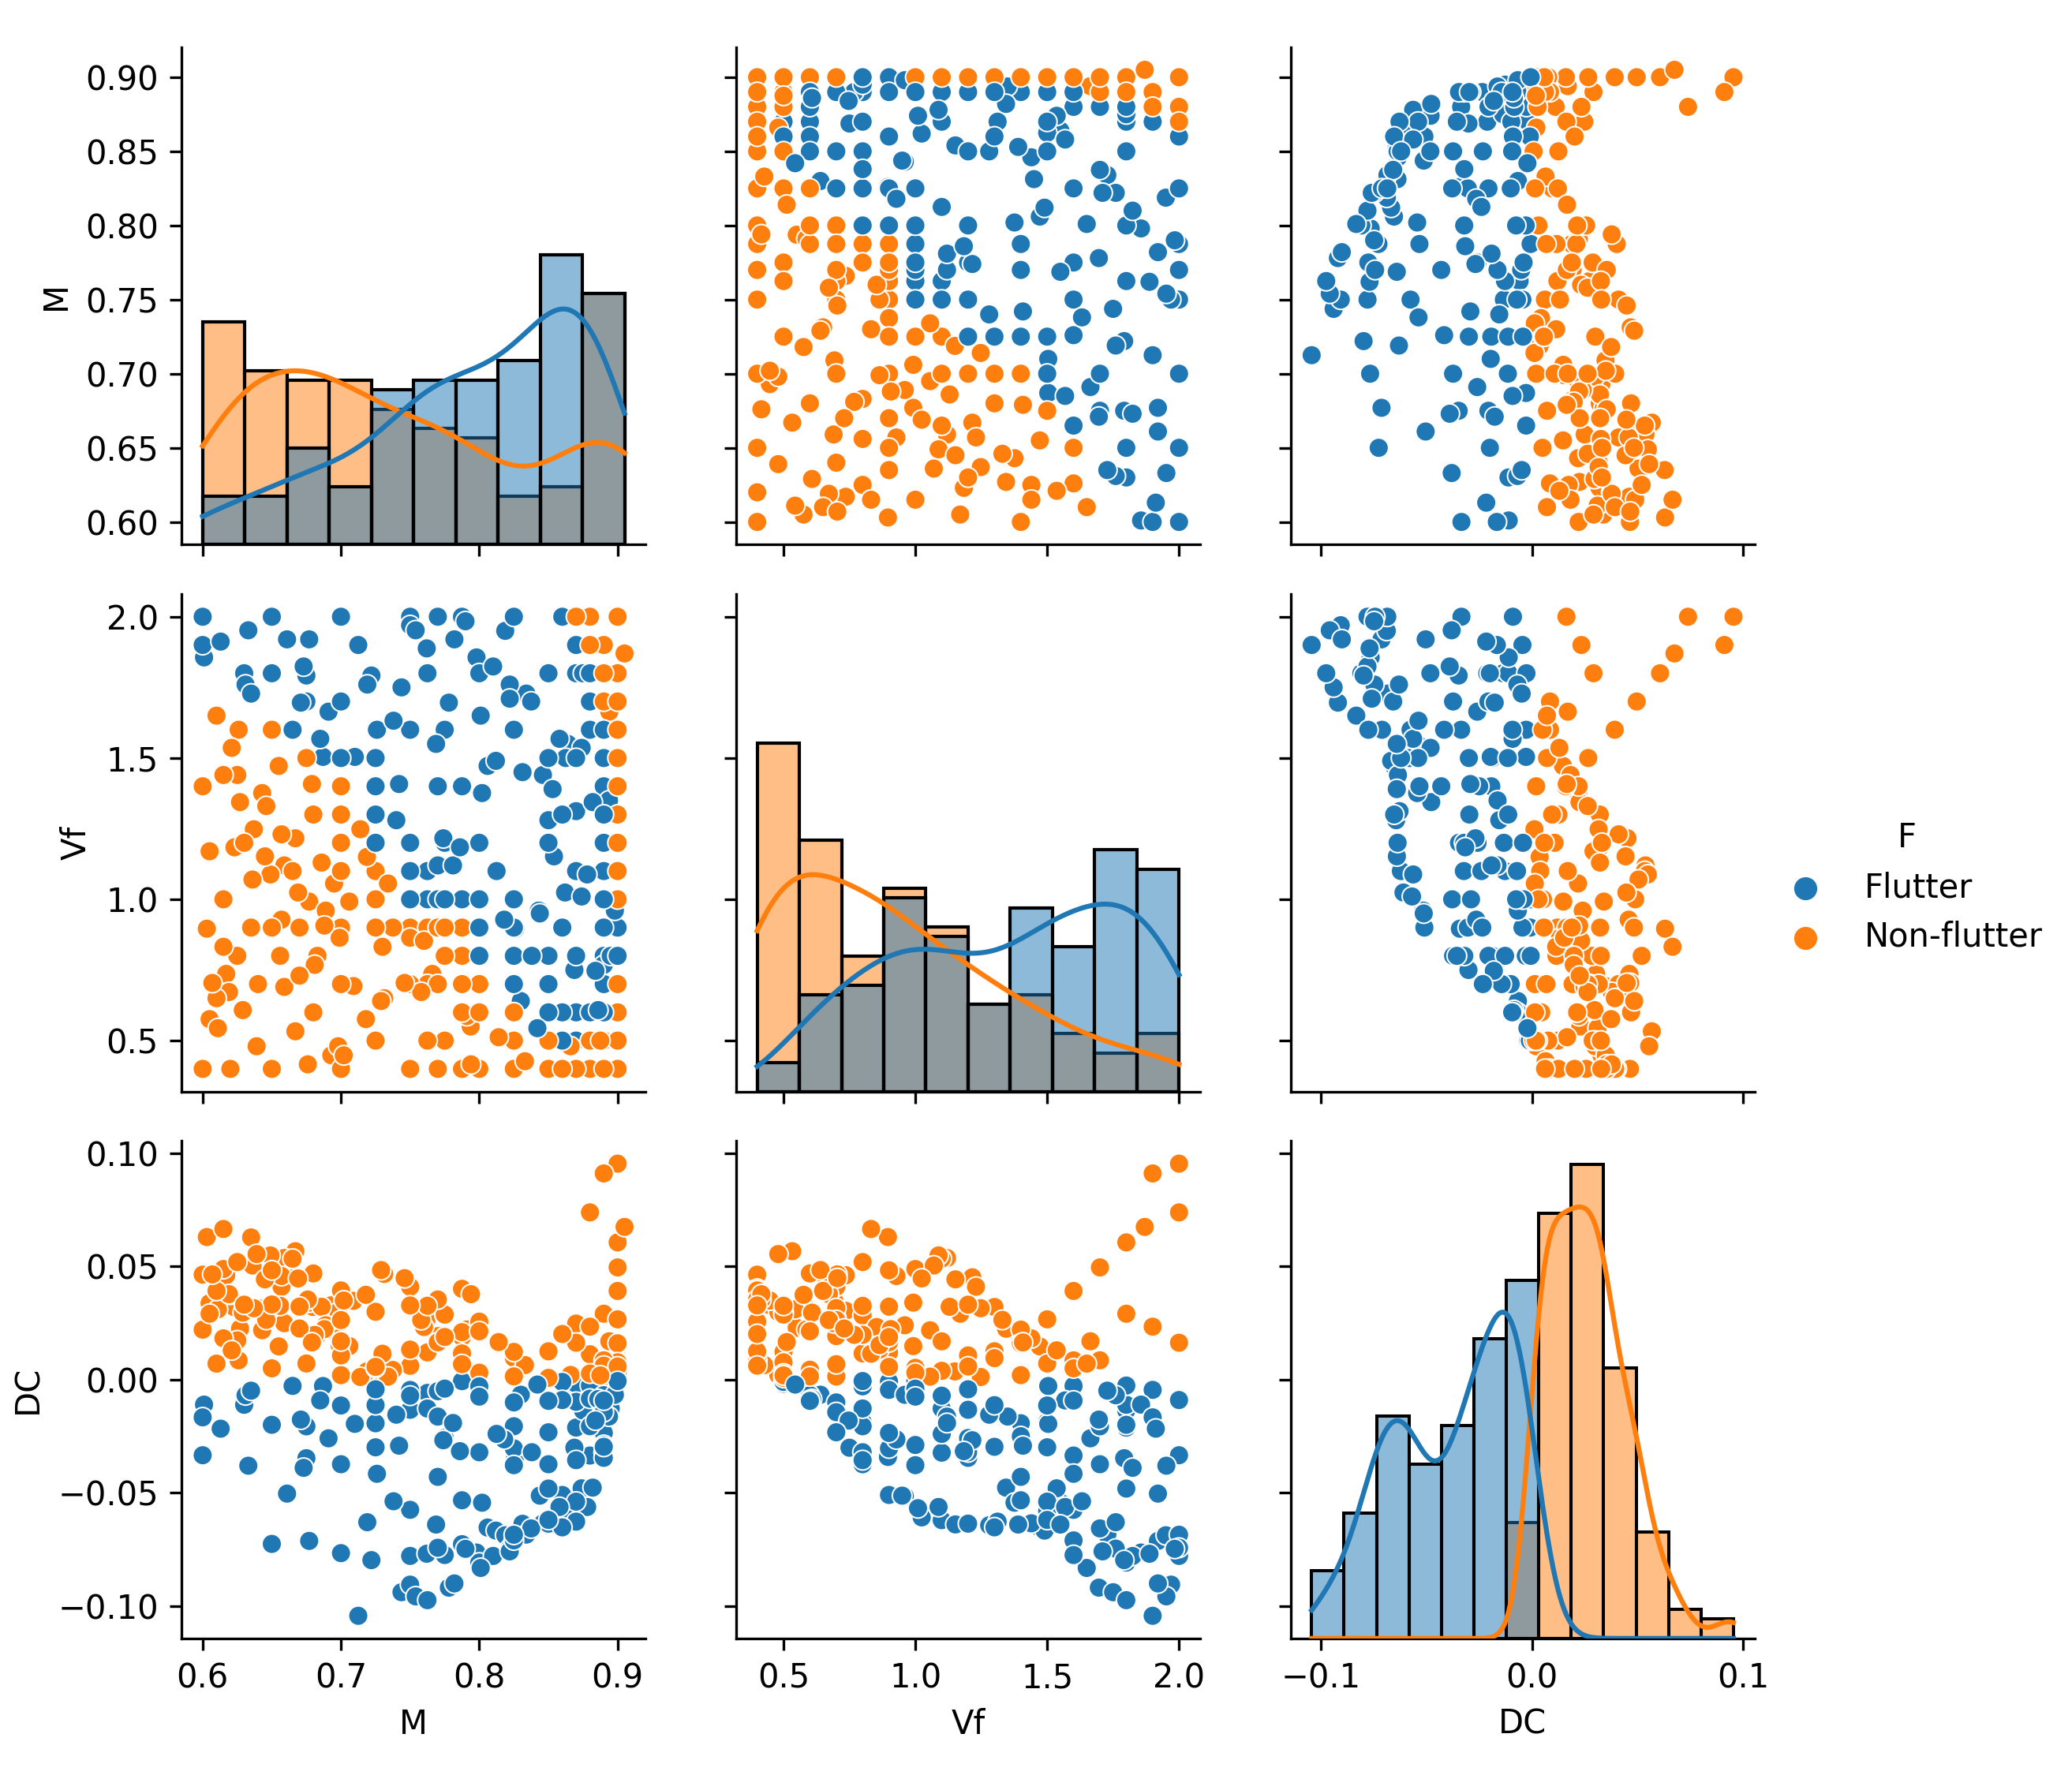
\includegraphics[width=0.8\textwidth]{graph/case3_data_dist_hue.png}
    \caption{Distribution of the data in case 3}
    \label{fig:case3_data_dist}
\end{figure}
Moreover, as we have only two inputs and an output, we may plot the data in a 3D scatter plot, as shown in Figure \ref{fig:case3_3d_scatter}.
\begin{figure}
    \centering
    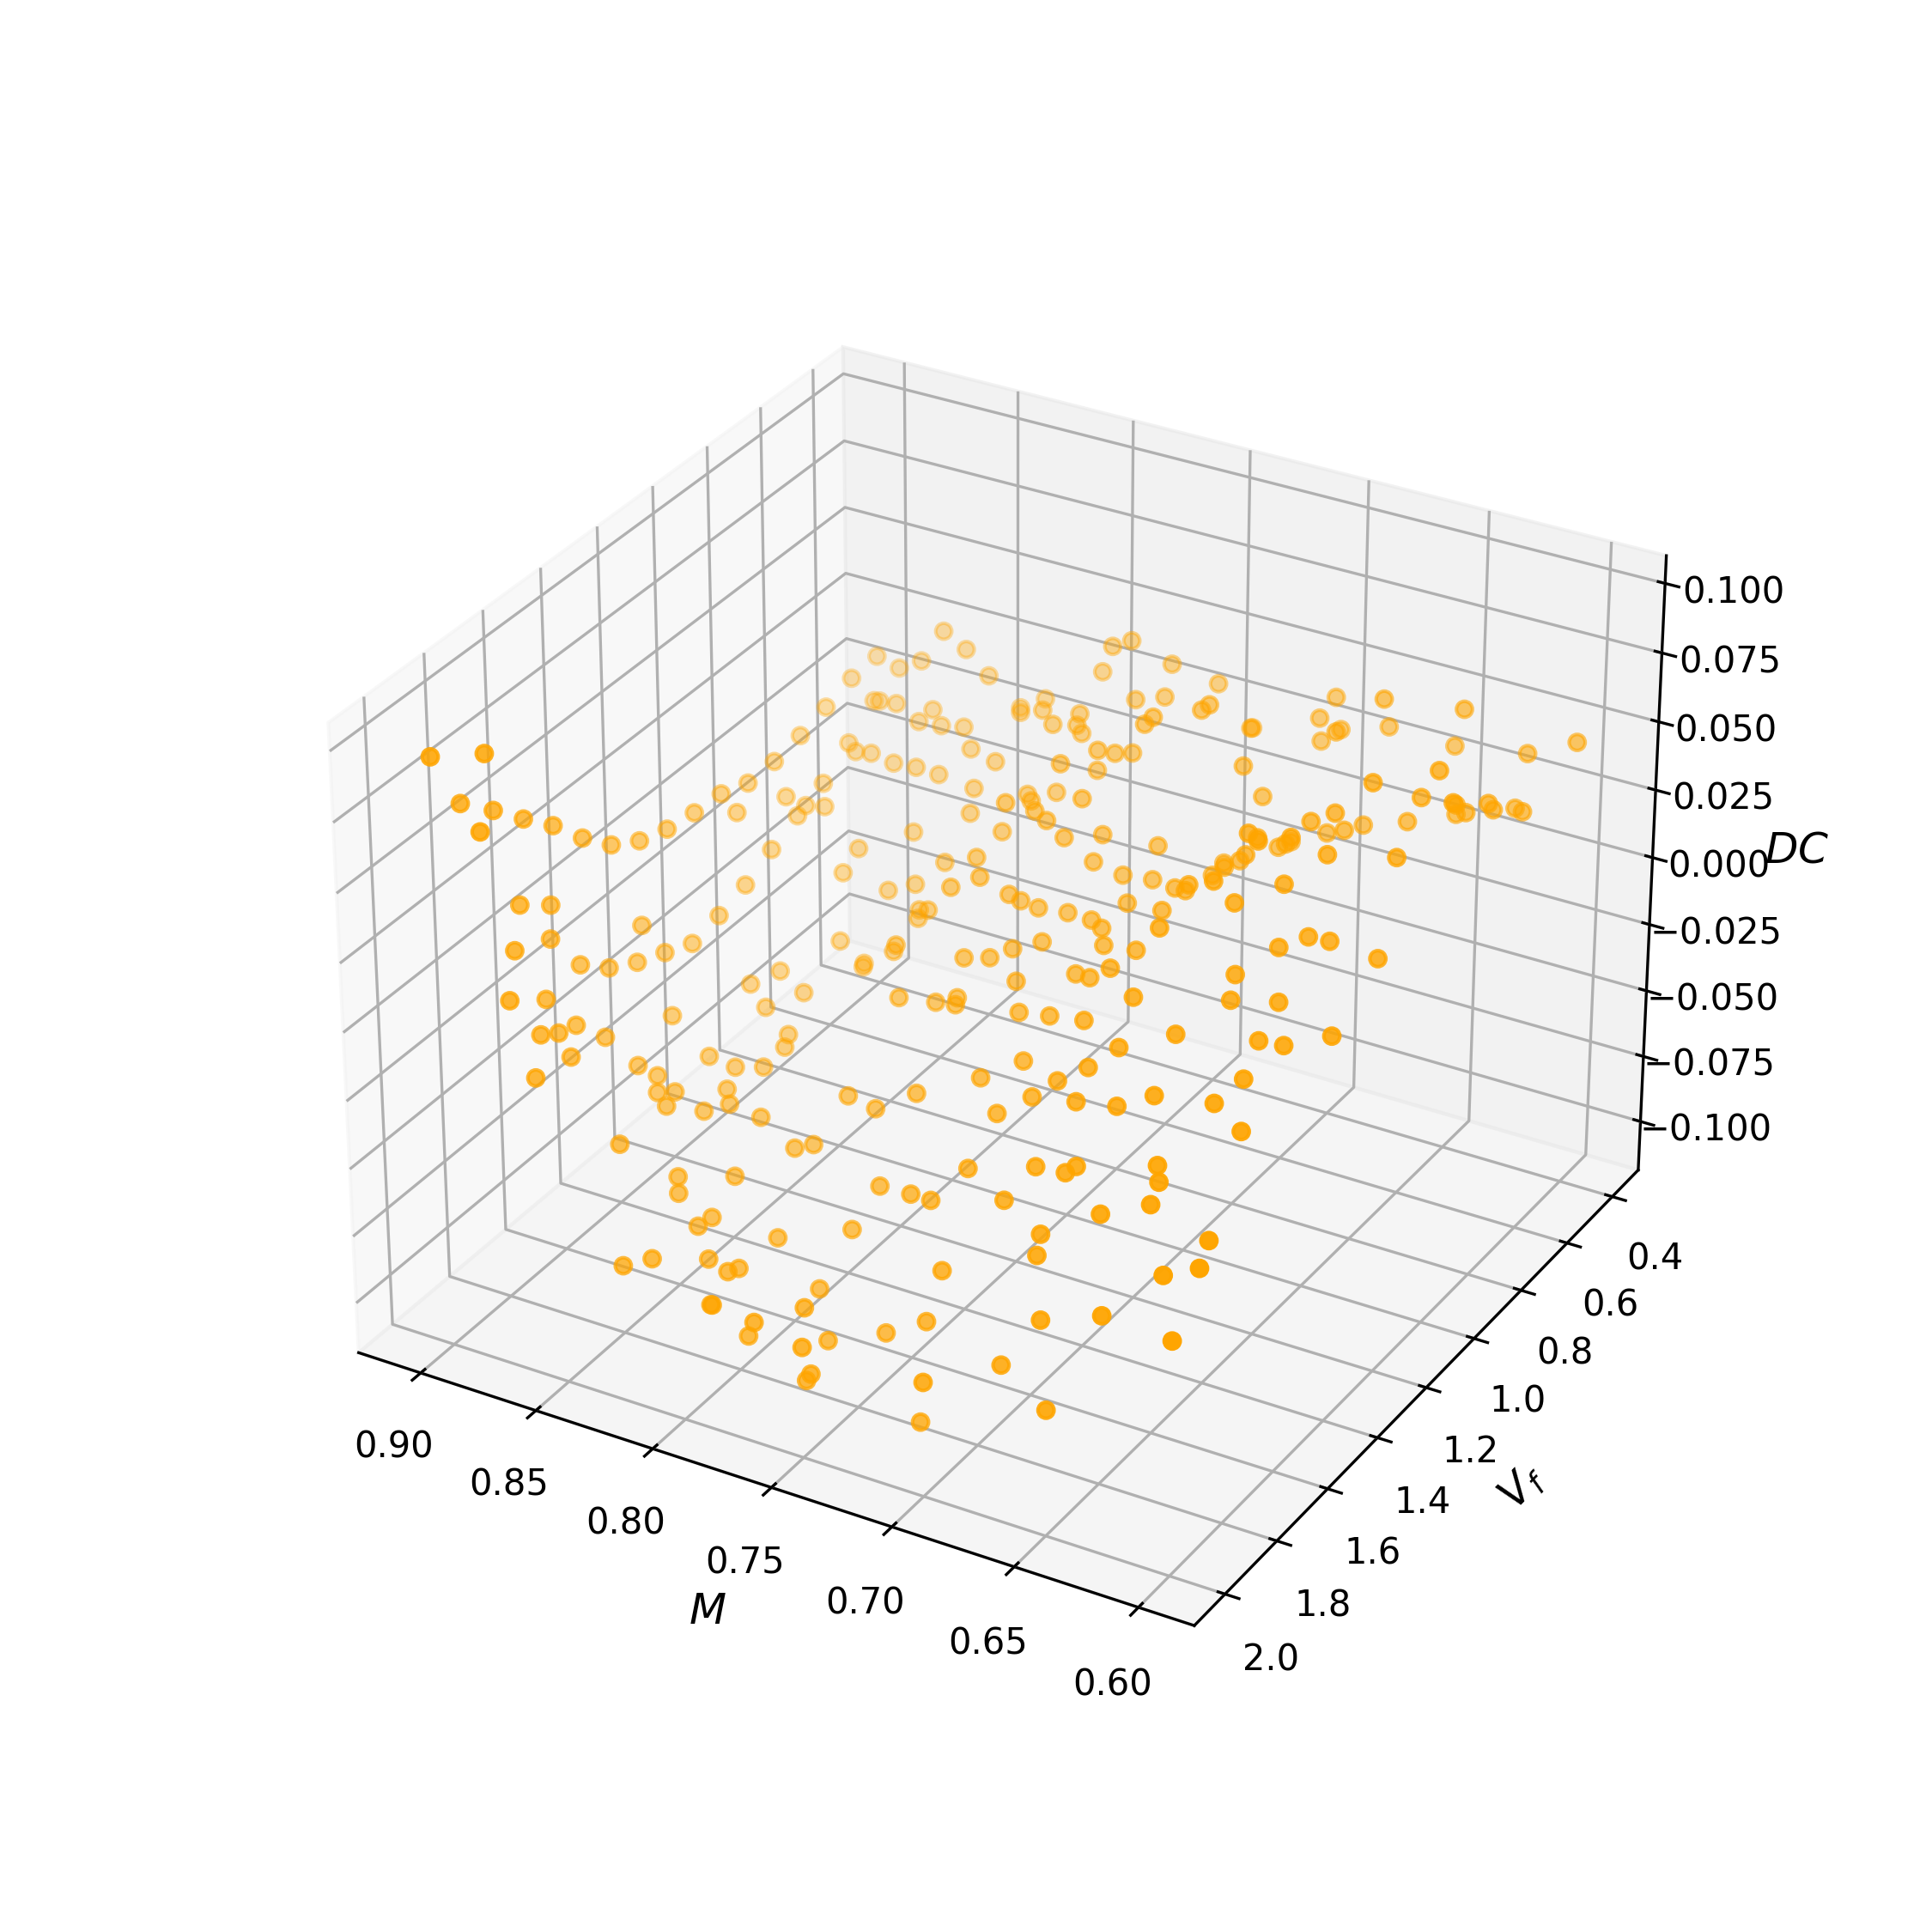
\includegraphics[width=0.5\textwidth]{graph/case3_3d_scatter.png}
    \caption{3D scatter plot of the sample data in case 3}
    \label{fig:case3_3d_scatter}
\end{figure}

\subsubsection{Model Selection}
Here, we have to predict a categorical value, so it's quite intuitive if we use a classification model. However, the classification of our target/response, $F$, is based on value of another column, $DC$, which can be predicted using a regression model. Therefore, we will use two approach in solving this problem:
\begin{enumerate}
    \item Predict $DC$ using a regression model, then obtain $F$ by classifying the result manually.
    \item Predict $F$ using a classification model.
\end{enumerate}

\subsubsection{Model Training and Evaluation}
\paragraph{Regression Approach}
We will use both linear regression and KNN regression to predict the value of $DC$.
\subparagraph{Linear Regression} Using the \eqref{eq:betaval}, the resulting coefficient for the linear regression model and the hypothesis testing is shown in Table \ref{tab:case3_ols_coef}. We can see that all $H_0$ is rejected and thus, all of the coefficients are significant. 
\begin{table}
    \centering
    \caption{ \label{tab:case3_ols_coef}OLS Coefficient for Linear Regression Model in Case 3}
    \begin{tabular}{lrrrrr}
        \toprule
        Beta &      Value &  Standard Error &  $t$-statistic &       $p$-value & Hypothesis Test Result \\
        \midrule
        0 &  0.158557 &        0.017985 &     8.816034 &  2.555677e-16 &              Reject $H_0$ \\
        1 & -0.145096 &        0.022156 &    -6.548710 &  3.543494e-10 &              Reject $H_0$ \\
        2 & -0.046859 &        0.004335 &   -10.808856 &  2.045755e-22 &              Reject $H_0$ \\
        \bottomrule
    \end{tabular}
\end{table}
With this model, we obtained a $R^2$ score of 0.39777 and an RSE score of 0.03249. This indicates that the relation between $DC$ and the inputs are not linear. We can see the resulting regression plane in Figure \ref{fig:case3_3d_linreg_plane}.
\begin{figure}
    \centering
    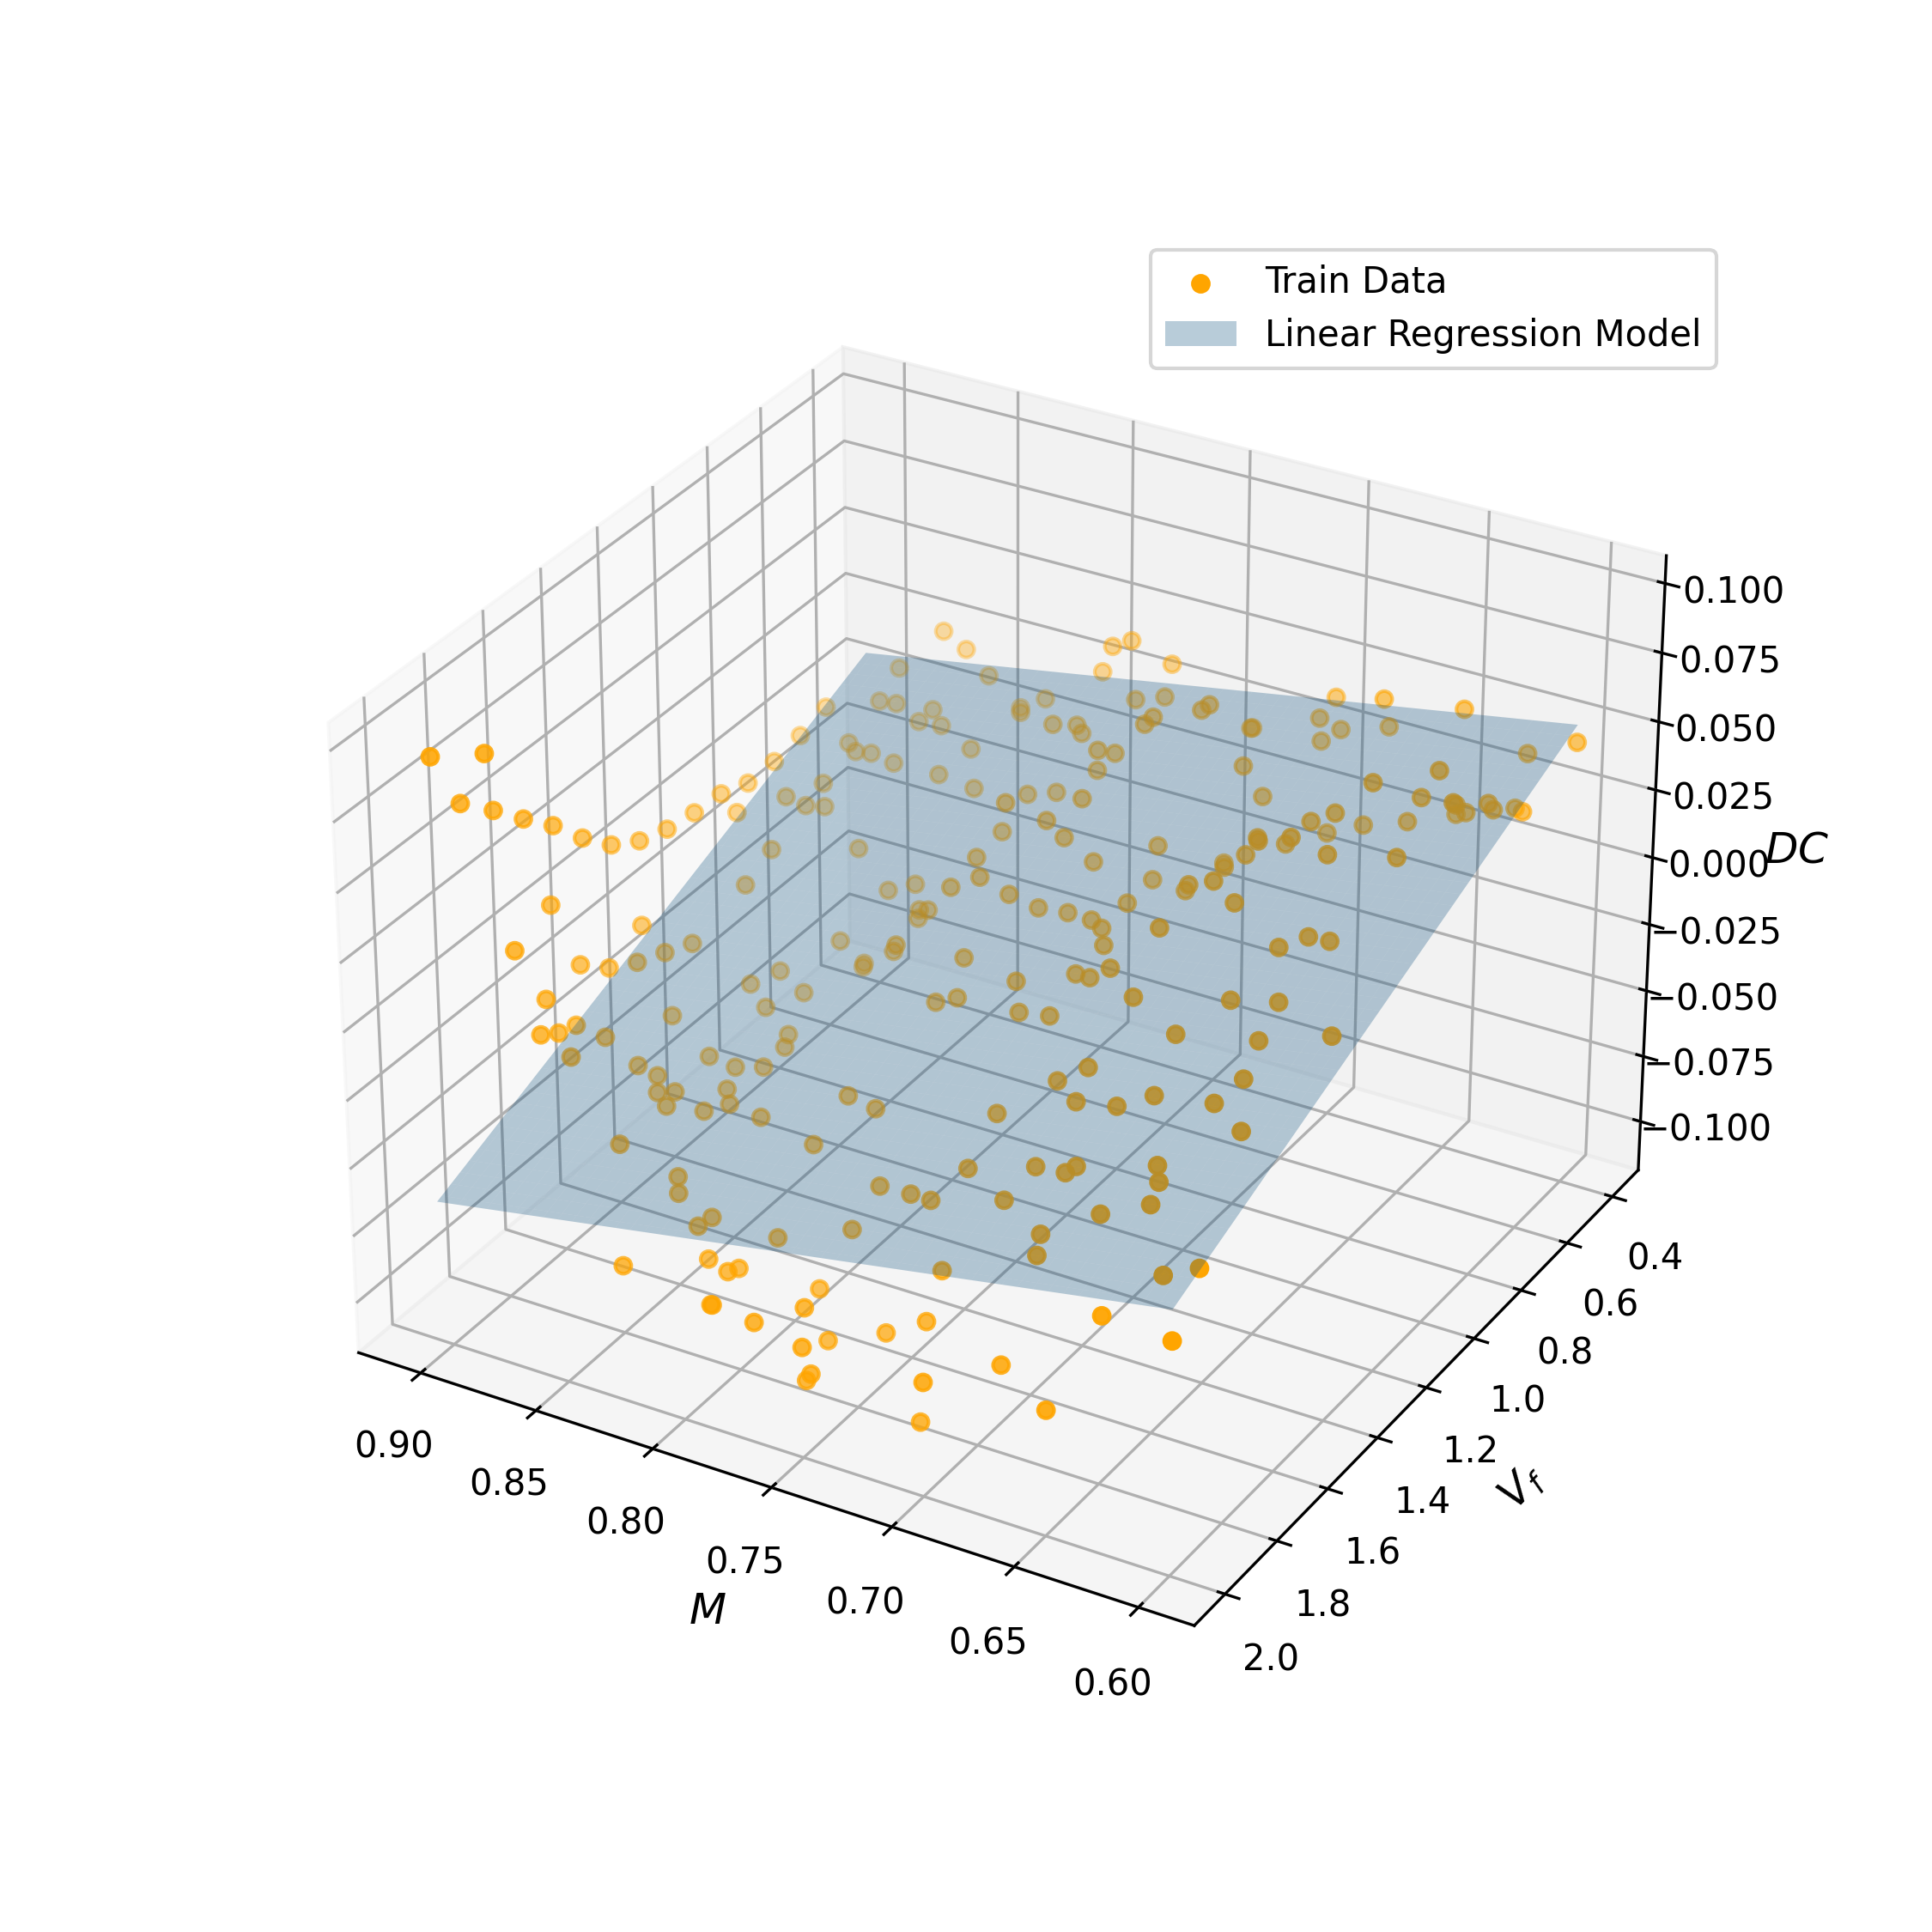
\includegraphics[width=0.5\textwidth]{graph/case3_3d_linreg_plane.png}
    \caption{Regression plane of the linear regression model in case 3}
    \label{fig:case3_3d_linreg_plane}
\end{figure}



\section{Conclusion}

\section{General Guidelines}

The following section outlines general (nonformatting) guidelines to follow, drawn from the original AIAA Manuscript Preparation Kit. These guidelines are applicable to all authors (except as noted), and include information on the policies and practices relevant to the publication of your manuscript.

\subsection{Publication by AIAA}
Your manuscript cannot be published by AIAA if:
\begin{enumerate}
\item It has been published previously or

\item The work contains copyright-infringing material or

\item An appropriate copyright statement has not yet been selected.
\end{enumerate}

\subsection{Paper Review and Visa Considerations}

It is the responsibility of the author to obtain any required government or company reviews for their papers in advance of publication. Start early to determine if the reviews are required; this process can take several weeks.

If you plan to attend an AIAA Forum, technical conference or professional development course held in the United States and you require a visa for travel, it is incumbent upon you to apply for a visa with the U.S.~embassy (consular division) or consulate with ample time for processing.  To avoid bureaucratic problems, AIAA strongly suggests that you submit your formal application to U.S.~ authorities a minimum of 120 days in advance of the date of anticipated travel.

Prospective conference and course attendees requiring a visa to travel to the United States should first contact

AIAA to request an official letter of invitation. This letter and a copy of the conference call for papers should be presented along with the required documentation to the U.S. consular officials as part of the formal application process.  AIAA cannot directly intervene with the U.S. Department of State, consular offices, or embassies on behalf of individuals applying for visas. A letter of invitation can be requested by completing the Visa Invitation Letter Request Form at \url{https://www.aiaa.org/Secondary.aspx?id=6258} or you may contact the Event Registrar at \url{invitation@aiaa.org} for more information.

\subsection{Control ID Number vs Paper Number}

Your paper was assigned a control ID number at the time you submitted your abstract. It is critical that you reference the tracking number and conference name when contacting AIAA regarding your submission. The control ID number is \emph{not} the final AIAA paper number. The paper number, which appears in the format AIAA-20XX-XXXX, will be used to refer to your paper in the program and in any publication format. It will not be assigned until shortly before the conference. \textbf{Do not include a paper number anywhere on your paper, as this number will be stamped automatically in the top right corner of your paper at the time of processing.}

\subsection{Copyright}

Before AIAA can print or publish any paper, the copyright information must be completed in the submission system. Failure to complete the electronic form correctly could result in your paper not being published. The following fields must be completed:

\begin{enumerate}
\item Clearance Statement
\item Non-Infringement Statement
\item Publication Status Statement
\item One Copyright Assignment Statement (Select either A, B, C, or D)
\end{enumerate}

Be sure to read the copyright statements carefully. AIAA requires a copyright transfer from the author(s) to AIAA or a license to publish and distribute your material; government authors can assert that the work is in the public domain. If you are not sure which copyright statement to use, contact your legal department. Refer to AIAA’s Rights and Permissions page at \url{www.aiaa.org} for more information; AIAA cannot help you determine which statement to use. Do not include a copyright statement anywhere on your paper. A hard copy of the form is found in the Author Kit for your reference. As you will be completing this form online, you do not need to fill out the hard-copy form. Do not include a copyright statement anywhere on your paper, and do not upload a copyright form with your paper. The correct statement will be stamped automatically at the time of processing.

\subsection{Submission Deadlines}

Manuscripts will be accepted for upload to the system from the receipt of the email invitation until the deadline set for the conference. You will be notified of the specific manuscript submission deadline in your acceptance letter, and the deadline will also be listed on the conference web page at AIAA. Please do not upload a draft version of your manuscript with the intent to upload a final version later. \textbf{Please review your manuscript very carefully before completing your submission to ensure that your paper is complete and final in all respects. Once the manuscript deadline has passed you will be locked out of the manuscript site so it is critical that you upload a final, carefully proofed document.}

Online conference proceedings will be made accessible to attendees who have registered for the ``full conference'' when the conference opens. Once the proceedings are published online, the conference papers will be considered the version of record and may not be removed or replaced. Changes to published papers can be made available through the Crossmark feature, where corrections and updates are accessed by clicking the Crossmark icon available on every paper published in Aerospace Research Central.

The opportunity to submit Crossmark updates will be provided to presenting authors starting the first day of the conference through 2000 hrs/8 pm Eastern Time, seven business days after the last day of the conference.  The proceedings will be updated with Crossmark updates shortly after that date.  

AIAA will NOT accept changes and/or change requests that solely correct grammatical errors, spelling errors, or errors in formatting.  All corrections should be for editorially significant changes where the change affects interpretation or crediting of the work.

To ensure conference quality, session chairs will enforce a ``no paper, no podium'' rule. This policy is intended to eliminate no-shows, to improve the quality of the conference for all participants, and to ensure that the published proceedings accurately represent the presentations made at a conference.

\section{Detailed Formatting Instructions}

The styles and formats for the AIAA Papers Template have been incorporated into the structure of this document. If you are using \LaTeX{}, please use this template to prepare your manuscript. A Microsoft Word template is also available from AIAA's website if you prefer to use Microsoft Word 2001 or later. Regardless of which program you use to prepare your manuscript, please use the formatting instructions contained in this document as a guide.

If you are using the AIAA Meeting Papers \LaTeX{} Template file to prepare your manuscript, you can simply type your own text over sections of this document, or cut and paste from another document and use the available markup styles. If you choose to cut and paste, select the text from your original document and choose Edit>Copy. (Do not select your title and author information, since the document spacing may be affected. It is a simple task to reenter your title and author information in the template.) Open the \LaTeX{} template file. Place your cursor in the text area of the template and select Edit>Paste. Please note that special formatting (e.g., subscripts, superscripts, italics) may be lost when you copy your text into the template. Use italics for emphasis; do not underline. Use the compiled \LaTeX{} pdf to see the most accurate representation of how your final paper will appear.

\subsection{Document Text}
The default font for AIAA papers is Times New Roman, 10-point size.  The first line of every paragraph should be indented, and all lines should be single-spaced. Default margins are 1'' on all sides. In the electronic version of this template, all margins and other formatting is preset. There should be no additional lines between paragraphs.

\begin{quoting}
Extended quotes, such as this example, are to be used when material being cited is longer than a few sentences, or the standard quotation format is not practical. In this \LaTeX template, the appropriate command environment is \verb|\begin{quoting}...\end{quoting}|. Extended quotes are to be in Times New Roman, 9-point font, indented 0.4'' and full justified.
\end{quoting}

\emph{NOTE:} If you are using the electronic \LaTeX{} template to format your manuscript, the required spacing and formatting will be applied automatically.

\subsection{Headings}
The title of your paper should be typed in bold, 24-point type, with capital and lower-case letters, and centered at the top of the page. The names of the authors, business or academic affiliation, city, and state/province should follow on separate lines below the title. The names of authors with the same affiliation can be listed on the same line above their collective affiliation information. Author names are centered, and affiliations are centered and in italic type immediately below the author names. The affiliation line for each author is to include that author’s city, state, and zip/postal code (or city, province, zip/postal code and country, as appropriate). The first-page footnotes (lower left-hand side) contain the job title and department name, street address/mail stop, and AIAA member grade for each author. Author email addresses may be included also.

Major headings (``sections'' in the \LaTeX{} template commands) are bold 11-point font, centered, and numbered with Roman numerals.

Subheadings (``subsections'' in the \LaTeX{} template commands) are bold, flush left, and numbered with capital letters. 

Sub-Subheadings (``subsubsections'' in the \LaTeX{} template commands) are italic, flush left, and numbered (1. 2. 3. etc.)


\subsection{Abstract}
The abstract should appear at the beginning of your paper. It should be one paragraph long (not an introduction) and complete in itself (no reference numbers). It should indicate subjects dealt with in the paper and state the objectives of the investigation. Newly observed facts and conclusions of the experiment or argument discussed in the paper must be stated in summary form; readers should not have to read the paper to understand the abstract. The abstract should be bold, indented 3 picas (1/2'') on each side, and separated from the rest of the document by blank lines above and below the abstract text..

\subsection{Nomenclature}
Papers with many symbols may benefit from a nomenclature list that defines all symbols with units, inserted between the abstract and the introduction. If one is used, it must contain all the symbology used in the manuscript, and the definitions should not be repeated in the text. In all cases, identify the symbols used if they are not widely recognized in the profession. Define acronyms in the text, not in the nomenclature.

\subsection{Footnotes and References}
Footnotes, where they appear, should be placed above the 1'' margin at the bottom of the page. To insert footnotes into the template, use the Insert>Footnote feature from the main menu as necessary. Numbered footnotes as formatted automatically in the template are acceptable, but superscript  symbols are the preferred AIAA style, *, $\dag$, $\ddag$, \S, \P, **, $\dag\dag$, $\ddag\ddag$, \S\S, etc.

List and number all references at the end of the paper. Corresponding bracketed numbers are used to cite references in the text \cite{vatistas1986reverse}, including citations that are an integral part of the sentence (e.g., ``It is shown in \cite{dornheim1996planetary} that\ldots '') or follow a mathematical expression: ``$A^{2} + B = C$ (Ref.~\cite{terster1997nasa}).'' For multiple citations, separate reference numbers with commas \cite{peyret2012computational,oates1997aerothermodynamics}, or use a dash to show a range \cite{volpe1994techniques,thompsonspacecraft,chi1993fluid,brandis2016nonequi}. Reference citations in the text should be in numerical order.

In the reference list, give all authors' names; do not use ``et al.''. Papers that have not been published should be cited as ``unpublished''; papers that have been submitted or accepted for publication should be cited as ``submitted for publication.'' Private communications and personal website should appear as footnotes rather than in the reference list.

References should be cited according to the standard publication reference style (for examples, see the ``References'' section of this template). Never edit titles in references to conform to AIAA style of spellings, abbreviations, etc. Names and locations of publishers should be listed; month and year should be included for reports and papers. For papers published in translation journals, please give the English citation first, followed by the original foreign language citation.

\subsection{Images, Figures and Tables}
All artwork, captions, figures, graphs, and tables will be reproduced exactly as submitted. Be sure to position any figures, tables, graphs, or pictures as you want them printed. AIAA will not be responsible for incorporating your figures, tables, etc. (Company logos and identification numbers are not permitted on your illustrations.)

Do not insert your tables and figures in text boxes. Figures should have no background, borders, or outlines. In the \LaTeX{} template, use the ``caption'' command to type caption text. Captions are bold with a single tab (no hyphen or other character) between the figure number and figure description.

% \begin{table}
% \caption{\label{tab:table1} Transitions selected for thermometry}
% \centering
% \begin{tabular}{lcccccc}
% \hline
% & Transition& & \multicolumn{2}{c}{}\\\cline{2-2}
% Line& $\nu''$& & $J'' $& Frequency, cm$^{-1}$& $FJ$, cm$^{-1}$& $G\nu $, cm$^{-1}$\\\hline
% a& 0& P$_{12}$& 2.5& 44069.416& 73.58& 948.66\\
% b& 1& R$_{2}$& 2.5& 42229.348& 73.41& 2824.76\\
% c& 2& R$_{21}$& 805& 40562.179& 71.37& 4672.68\\
% d& 0& R$_{2}$& 23.5& 42516.527& 1045.85& 948.76\\
% \hline
% \end{tabular}
% \end{table}


\begin{figure}[hbt!]
\centering
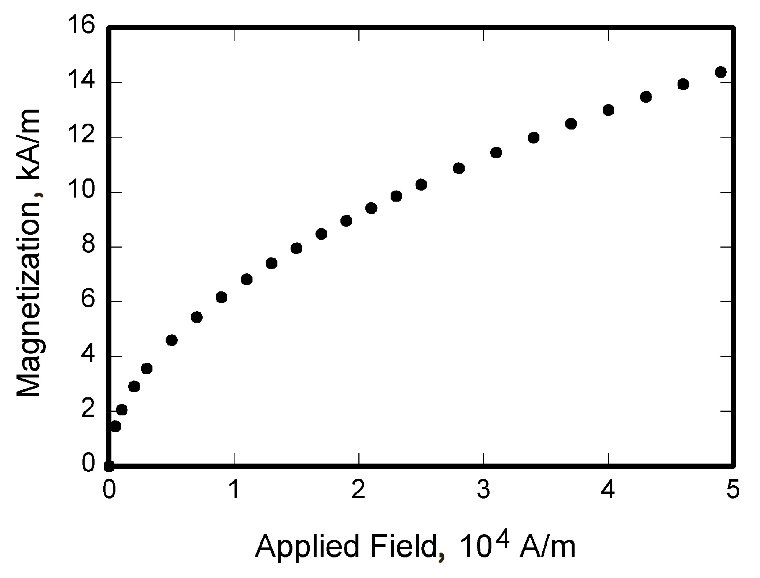
\includegraphics[width=.5\textwidth]{graph}
\caption{Magnetization as a function of applied fields.}
\end{figure}

Place figure captions below all figures; place table titles above the tables. If your figure has multiple parts, include the labels ``a),'' ``b),'' etc. below and to the left of each part, above the figure caption. Please verify that the figures and tables you mention in the text actually exist. \emph{Please do not include captions as part of the figures, and do not put captions in separate text boxes linked to the figures.} When citing a figure in the text, use the abbreviation ``Fig.'' except at the beginning of a sentence. Do not abbreviate ``Table.'' Number each different type of illustration (i.e., figures, tables, images) sequentially with relation to other illustrations of the same type.

Figure axis labels are often a source of confusion. Use words rather than symbols. As in the example to the right, write the quantity ``Magnetization'' rather than just ``M.'' Do not enclose units in parenthesis, but rather separate them from the preceding text by commas. Do not label axes only with units. As in Fig.~1, for example, write ``Magnetization, \si[per-mode=symbol]{\ampere\per\meter},'' not just ``A/m.'' Do not label axes with a ratio of quantities and units. For example, write ``Temperature, K,'' not ``Temperature/K.''

Multipliers can be especially confusing. Write ``Magnetization, \si[per-mode=symbol]{\kilo\ampere\per\meter}'' or ``Magnetization, \SI[per-mode=symbol]{e3}{\ampere\per\meter}.'' Do not write ``Magnetization (A/m) x 1000'' because the reader would not then know whether the top axis label in Fig.~1 meant 16000 A/m or 0.016 A/m. Figure labels must be legible, and all text within figures should be uniform in style and size, no smaller than 8-point type.

\subsection{Equations, Numbers, Symbols, and Abbreviations}
Equations are numbered consecutively, with equation numbers in parentheses flush right, as in Eq.~\eqref{sample:equation}. Insert a blank line above and below the equation. To insert an equation into the \LaTeX{} document, use the \verb|\begin{equation}...\end{equation}| command environment.

A sample equation is included here, formatted using the preceding instructions. To make your equation more compact, you can use the solidus (/), the exp function, or appropriate exponents. Use parentheses to avoid ambiguities in denominators.

\begin{equation}
\label{sample:equation}
\int^{r_2}_0 F(r,\varphi){\rm d}r\,{\rm d}\varphi = [\sigma r_2/(2\mu_0)]\int^{\infty}_0\exp(-\lambda|z_j-z_i|)\lambda^{-1}J_1 (\lambda r_2)J_0 (\lambda r_i\,\lambda {\rm d}\lambda)
\end{equation}

Be sure that the symbols in your equation are defined before the equation appears, or immediately following. Italicize symbols ($T$ might refer to temperature, but T is the unit tesla). Refer to ``Eq.~(1),'' not ``(1)'' or ``equation (1)'' except at the beginning of a sentence: ``Equation (1) is\ldots'' Equations can be labeled other than ``Eq.'' should they represent inequalities, matrices, or boundary conditions. If what is represented is really more than one equation, the abbreviation ``Eqs.'' can be used.

Define abbreviations and acronyms the first time they are used in the text, even after they have already been defined in the abstract. Very common abbreviations such as AIAA, SI, ac, and dc do not have to be defined. Abbreviations that incorporate periods should not have spaces: write ``P.R.,'' not ``P.~R.'' Delete periods between initials if the abbreviation has three or more initials; e.g., U.N.~but ESA. Do not use abbreviations in the title unless they are unavoidable (for instance, ``AIAA'' in the title of this article).

\subsection{General Grammar and Preferred Usage}
Use only one space after periods or colons. Hyphenate complex modifiers: ``zero-field-cooled magnetization.'' Avoid dangling participles, such as, ``Using Eq.~(1), the potential was calculated.'' [It is not clear who or what used Eq.~(1).] Write instead ``The potential was calculated using Eq.~(1),'' or ``Using Eq.~(1), we calculated the potential.''

Insert a zero before decimal points: ``0.25,'' not ``.25.'' Use ``\si{\centi\meter\squared}'' not ``cc.'' Indicate sample dimensions as ``$\SI{0.1}{\centi\meter} \times \SI{0.2}{\centi\meter}$,'' not ``$0.1 \times \SI{0.2}{\centi\meter\squared}$.'' The preferred abbreviation for ``seconds'' is ``s,'' not ``sec.'' Do not mix complete spellings and abbreviations of units: use ``\si[per-mode=symbol]{\weber\per\meter\squared}'' or ``webers per square meter,'' not ``webers/m$^2$.'' When expressing a range of values, write ``7 to 9'' or ``7--9,'' not ``7$\sim$9.''

A parenthetical statement at the end of a sentence is punctuated outside of the closing parenthesis (like this). (A parenthetical sentence is punctuated within parenthesis.) In American English, periods and commas are placed within quotation marks, like ``this period.'' Other punctuation is ``outside''! Avoid contractions; for example, write ``do not'' instead of ``don’t.'' The serial comma is preferred: ``A, B, and C'' instead of ``A, B and C.''

If you wish, you may write in the first person singular or plural and use the active voice (``I observed that\ldots'' or ``We observed that\ldots'' instead of ``It was observed that\ldots''). Remember to check spelling. If your native language is not English, please ask a native English-speaking colleague to proofread your paper.

Be aware of the different meanings of the homophones ``affect'' (usually a verb) and ``effect'' (usually a noun), ``complement'' and ``compliment,'' ``discreet'' and ``discrete,'' ``principal'' (e.g., ``principal investigator'') and ``principle'' (e.g., ``principle of measurement''). Do not confuse ``imply'' and ``infer.''

The word ``data'' is plural, not singular (i.e., ``data are,'' not ``data is''). The subscript for the permeability of vacuum $\mu_0$ is zero, not a lowercase letter ``o.'' The term for residual magnetization is ``remanence''; the adjective is ``remanent''; do not write ``remnance'' or ``remnant.'' The word ``micrometer'' is preferred over ``micron'' when spelling out this unit of measure. A graph within a graph is an ``inset,'' not an ``insert.'' The word ``alternatively'' is preferred to the word ``alternately'' (unless you really mean something that alternates). Use the word ``whereas'' instead of ``while'' (unless you are referring to simultaneous events). Do not use the word ``essentially'' to mean ``approximately'' or ``effectively.'' Do not use the word ``issue'' as a euphemism for ``problem.'' When compositions are not specified, separate chemical symbols by en-dashes; for example, ``NiMn'' indicates the intermetallic compound \ce{Ni_{0.5}Mn_{0.5}} whereas ``Ni--Mn'' indicates an alloy of some composition \ce{Ni_{x}Mn_{1-x}}.

Be aware of the different meanings of the homophones ``affect'' (usually a verb) and ``effect'' (usually a noun), ``complement'' and ``compliment,'' ``discreet'' and ``discrete,'' ``principal'' (e.g., ``principal investigator'') and ``principle'' (e.g., ``principle of measurement''). Do not confuse ``imply'' and ``infer.''

Prefixes such as ``non,'' ``sub,'' ``micro,'' ``multi,'' and ``"ultra'' are not independent words; they should be joined to the words they modify, usually without a hyphen. There is no period after the ``et'' in the abbreviation ``et al.'' The abbreviation ``i.e.,'' means ``that is,'' and the abbreviation ``e.g.,'' means ``for example'' (these abbreviations are not italicized).


\section{Conclusion}
A conclusion section is not required, though it is preferred. Although a conclusion may review the main points of the paper, do not replicate the abstract as the conclusion. A conclusion might elaborate on the importance of the work or suggest applications and extensions. \textit{Note that the conclusion section is the last section of the paper that should be numbered. The appendix (if present), acknowledgment, and references should be listed without numbers.}


\section*{Appendix}

An Appendix, if needed, should appear before the acknowledgments.

\section*{Acknowledgments}
An Acknowledgments section, if used, \textbf{immediately precedes} the References. Sponsorship information and funding data are included here. The preferred spelling of the word ``acknowledgment'' in American English is without the ``e'' after the ``g.'' Avoid expressions such as ``One of us (S.B.A.) would like to thank\ldots'' Instead, write ``F.~A.~Author thanks\ldots'' Sponsor and financial support acknowledgments are also to be listed in the ``acknowledgments'' section.

\bibliographystyle{new-aiaa}
\bibliography{reference}

\end{document}
